\documentclass[11pt,a4paper]{article}

% ===================== Codificación y fuentes =====================
\usepackage[utf8]{inputenc}
\usepackage[T1]{fontenc}

% ===================== Página y utilidades ========================
\usepackage[left=2.5cm,right=2.5cm,top=2.5cm,bottom=2.5cm]{geometry}
\usepackage{array}
\usepackage{enumitem}
\usepackage{graphicx}
\usepackage{xcolor}
\usepackage{titlesec}
\usepackage{fancyhdr}
\usepackage[most]{tcolorbox}
\usepackage{hyperref}
\usepackage{booktabs}

% ===================== Etiquetas en español (sin babel) ===========
\renewcommand{\contentsname}{Índice}
\renewcommand{\figurename}{Figura}
\renewcommand{\tablename}{Tabla}
\renewcommand{\refname}{Bibliografía}

% ===================== Escala de grises (sin color) ================
\definecolor{negro}{RGB}{0,0,0}
\definecolor{gris}{RGB}{90,90,90}
\definecolor{grisclaro}{RGB}{150,150,150}
\definecolor{fillgray}{RGB}{175,175,175}

% ===================== Hipervínculos (negro) =======================
\hypersetup{colorlinks=true, linkcolor=negro, urlcolor=negro, citecolor=negro}

% ===================== Estilo de títulos ===========================
\titleformat{\section}{\large\bfseries\color{negro}}{\thesection.}{0.5em}{}
\titleformat{\subsection}{\normalsize\bfseries\color{negro}}{\thesubsection}{0.5em}{}
\titlespacing*{\section}{0pt}{1.4em}{0.4em}
\titlespacing*{\subsection}{0pt}{1.0em}{0.3em}

% ===================== Pie de página ===============================
\pagestyle{fancy}
\fancyhf{}
\fancyfoot[L]{\footnotesize\color{gris}Magíster en Ciencia de Datos e Inteligencia Artificial}
\fancyfoot[R]{\footnotesize\color{gris}\thepage}
\renewcommand{\headrulewidth}{0pt}
\renewcommand{\footrulewidth}{0.4pt}

% ===================== Comandos del docente ========================
\newcommand{\guia}[1]{{\small\itshape\color{gris}#1}\par\vspace{0.15em}}
\newcommand{\resp}{{\footnotesize\itshape\color{fillgray}[\,Desarrollen aquí\,]}\par\vspace{1.1em}}

% Caja de información de la evaluación (escala de grises):
\newtcolorbox{infobox}[1][Información de la evaluación]{colback=black!3,colframe=negro,
  fonttitle=\bfseries,coltitle=white,title={#1},boxrule=0.6pt,arc=1pt,
  left=8pt,right=8pt,top=6pt,bottom=6pt,breakable}

% Caja de conexión con evaluaciones previas (gris, sin color):
\newtcolorbox{conexionbox}[1][Conexión con evaluaciones anteriores]{colback=black!6,colframe=gris,
  fonttitle=\bfseries,coltitle=white,title={#1},boxrule=0.6pt,arc=1pt,
  left=8pt,right=8pt,top=6pt,bottom=6pt,breakable}

% ===================== Datos del grupo (COMPLETAR) ==================
\newcommand{\proyTitulo}{Predicción de riesgo de enfermedad coronaria a 10 años}
\newcommand{\proyIntegrantes}{Felipe Díaz Toro, Pablo Ríos Passteni, Guillermo Subiabre Chacón, Ninoska Yévenes Hernández}
\newcommand{\proyDataset}{Framingham Heart Study (Riesgo Cardiovascular)}
\newcommand{\proyDocente}{Jean Paul Maidana}
\newcommand{\proyFecha}{«dd/mm/aaaa»}
\newcommand{\proyRepo}{\url{https://github.com/fdiaztoro/proyecto-grupo3-mcdi501}}

\setlength{\parindent}{0pt}
\setlength{\parskip}{0.35em}

\begin{document}
\pagenumbering{gobble}

\thispagestyle{empty}
\begin{center}
\vspace*{1.0cm}

\includegraphics[height=4.4cm]{logo_unab.png}\\[1.3cm]

{\footnotesize\color{gris}\MakeUppercase{Magíster en Ciencia de Datos e Inteligencia Artificial}}\\[0.15cm]
{\footnotesize\color{grisclaro}MCDI501: Estadística Computacional para la Toma de Decisiones}\\[2.0cm]

{\Large\bfseries\color{negro} Evaluación Formativa 2}\\[0.45cm]
{\large\color{negro} Modelamiento Predictivo (práctica)}\\[1.0cm]

{\small\itshape\color{gris} Notebook grupal \textperiodcentered\ 0\,\% (formativa)}
\end{center}

\vspace{1.6cm}

\begin{flushleft}
\setlength{\extrarowheight}{5pt}
\begin{tabular}{@{}>{\bfseries\color{negro}}l @{\hspace{0.6em}} p{0.72\linewidth}@{}}
Título del proyecto: & \proyTitulo \\
Integrantes:         & \proyIntegrantes \\
Dataset:             & \proyDataset \\
Docente:             & \proyDocente \\
Fecha:               & \proyFecha \\
Repositorio GitHub:  & \proyRepo \\
\end{tabular}
\end{flushleft}

\clearpage
\pagenumbering{arabic}
\begin{infobox}
\textbf{Fase del proyecto:} Fase 3: Desarrollo del proyecto\\
\textbf{Modalidad:} Grupal\qquad\textbf{Ponderación:} 0\,\% (formativa)\\
\textbf{Entregable:} Notebook \texttt{.ipynb} ejecutable, con síntesis final en Markdown\\
\textbf{Resultado de aprendizaje (RA3):} evaluar modelos de regresión para problemas de predicción y clasificación en contextos de negocio o ingeniería.\\
\textbf{Indicadores:} ID3.1, ID3.2.\\
\textbf{Prerrequisito:} Sumativas 1 y 2 completadas (usarán sus resultados).
\end{infobox}
\begin{conexionbox}
Esta práctica formativa \textbf{no es independiente}: requiere el uso explícito de los resultados de S1 y S2 (selección de variables, tratamiento de outliers, correlaciones validadas y parámetros robustos), y prepara directamente la Evaluación Sumativa 3.
\end{conexionbox}

\vspace{0.5em}
\tableofcontents
\newpage

\section{Preparación de datos para modelamiento}
\guia{(21 pts) Carguen el dataset utilizado en evaluaciones anteriores; documenten explícitamente hallazgos de S1 (correlaciones con la variable objetivo, faltantes, outliers) y de S2 (correlaciones estables, parámetros robustos). Apliquen una estrategia básica de tratamiento de faltantes justificada, dividan en train/test (70/30) y estandaricen variables numéricas cuando corresponda.}

\subsection{Hallazgos de S1 y S2}
El punto de partida no es el dato crudo, sino lo aprendido en S1 (exploración e inferencia) y S2 (validación con remuestreo).

\begin{center}
\small
\begin{tabular}{@{}lrl@{}}
\toprule
\textbf{Variable} & \textbf{$r$ con CHD (S1)} & \textbf{IC bootstrap 95\,\% (S2)} \\
\midrule
Edad                     & 0,225 & [0,197; 0,254] \\
Presión sistólica        & 0,216 & [0,183; 0,250] \\
Hipertensión prevalente  & 0,178 & no validada en S2 \\
Glucosa                  & 0,126 & no validada en S2 \\
Diabetes                 & 0,097 & no validada en S2 \\
Sexo masculino           & 0,088 & no validada en S2 \\
Colesterol total         & 0,082 & no validada en S2 \\
IMC                      & 0,075 & no validada en S2 \\
Cigarrillos por día      & 0,058 & no validada en S2 \\
\bottomrule
\end{tabular}
\end{center}

Las variables más asociadas con CHD son la edad ($r=0,225$) y la presión sistólica ($r=0,216$); S2 confirmó que ambas son estables, con IC bootstrap estrechos que no incluyen el cero. S2 solo validó con remuestreo estas dos correlaciones: las demás candidatas cuentan únicamente con el valor puntual de S1, sin ese respaldo adicional, y se declara explícitamente en la tabla. Todas las correlaciones son modestas (máximo 0,23), lo esperable en un fenómeno multifactorial a 10 años.

Hay faltantes en siete variables, ninguna sobre el 10\,\%: glucosa concentra la mayoría (388 casos, 9,2\,\%), seguida de educación (105, 2,5\,\%); los 29 faltantes de cigarrillos por día (0,7\,\%) son todos fumadores actuales. La regla de Tukey marca 3,0\,\% de valores extremos en presión sistólica, 4,9\,\% en glucosa, 0,3\,\% en cigarrillos por día y 0\,\% en edad; S1 mostró que son plausibles (glucosas $\geq$200\,mg/dL corresponden a personas diabéticas), por lo que no se eliminan.

\subsection{Tratamiento de faltantes, partición y estandarización}
Estrategia simple, en este orden: (1) partición 70/30 estratificada por \texttt{TenYearCHD}, (2) tope de la glucosa, (3) imputación con medianas y (4) estandarización. Todo se calcula con el conjunto de entrenamiento y se aplica al de prueba, para evitar fuga de información.

La partición deja 2.966 participantes en train y 1.272 en test, con prevalencia de CHD casi idéntica (15,21\,\% y 15,17\,\%). La glucosa se acota al percentil 99 de train (187,1\,mg/dL), calculado solo con el 70\,\% de los datos. Los faltantes se imputan con la mediana de train; en cigarrillos por día se usa la mediana de los \textbf{fumadores} de train (20 cigarrillos/día), porque los 29 faltantes son fumadores actuales y la mediana general es 0, que los habría tratado como no fumadores. Tras estandarizar, los cinco predictores quedan con media 0 y desviación 1 en train, de modo que sus coeficientes serán comparables entre sí.

\section{Modelo de regresión logística}
\guia{(30 pts) Seleccionen 3 a 5 variables predictoras basándose en S1 y S2, justificando cada elección. Ajusten el modelo, presenten el resumen e interpreten coeficientes, odds ratios y significancia estadística. Realicen un diagnóstico básico mediante VIF y documenten problemas de multicolinealidad si los detectan.}

\subsection{Selección de variables}
Se seleccionan cinco predictores con un criterio doble: que la asociación con CHD aparezca en S1 y, cuando S2 la validó, que resista el remuestreo: \textbf{edad}, \textbf{presión sistólica}, \textbf{glucosa}, \textbf{sexo masculino} y \textbf{cigarrillos por día}. Se excluyen la presión diastólica y la hipertensión prevalente ($r=0,78$ y $r=0,70$ con la sistólica, S2), diabetes (solapada con glucosa, $r=0,62$) y colesterol total/IMC (asociaciones débiles, 0,082 y 0,075). Con unos 451 casos de CHD en train hay cerca de 90 por predictor, margen amplio para cinco variables.

\subsection{Ajuste e interpretación}
El modelo logístico (\texttt{statsmodels.Logit}) sobre los cinco predictores estandarizados mejora de forma clara sobre el nulo (LLR $p<0,001$) y explica una fracción moderada de la variación (pseudo $R^2=0,117$).

\begin{center}
\small
\begin{tabular}{@{}lrrrc@{}}
\toprule
\textbf{Variable} & \textbf{Coef.} & \textbf{Odds Ratio} & \textbf{$p$-valor} & \textbf{Sig. ($\alpha=0,05$)} \\
\midrule
Constante            & $-1,991$ & 0,137 & $<0,001$ & Sí \\
Edad                  & 0,608    & 1,837 & $<0,001$ & Sí \\
Presión sistólica     & 0,404    & 1,497 & $<0,001$ & Sí \\
Sexo masculino        & 0,201    & 1,223 & 0,0005   & Sí \\
Cigarrillos por día   & 0,291    & 1,338 & $<0,001$ & Sí \\
Glucosa               & 0,154    & 1,166 & 0,0008   & Sí \\
\bottomrule
\end{tabular}
\end{center}

Los cinco predictores son significativos al 5\,\% ($p\leq0,0008$). Como están estandarizados, cada odds ratio se lee ``por cada desviación estándar de aumento en la variable, manteniendo las demás constantes''. La edad tiene el mayor efecto (OR = 1,84), coherente con ser la variable más correlacionada en S1; le sigue la presión sistólica (OR = 1,50). Cigarrillos por día (OR = 1,34) y glucosa (OR = 1,17) también aumentan el riesgo: el tabaquismo sí aporta en el modelo multivariable, aunque S2 no distinguiera de cero su correlación marginal. El sexo masculino (OR = 1,22) también es significativo.

\subsection{Diagnóstico: VIF}
\begin{center}
\small
\begin{tabular}{@{}lr@{}}
\toprule
\textbf{Variable} & \textbf{VIF} \\
\midrule
Edad                & 1,23 \\
Presión sistólica   & 1,20 \\
Sexo masculino      & 1,12 \\
Cigarrillos por día & 1,17 \\
Glucosa             & 1,03 \\
\bottomrule
\end{tabular}
\end{center}

Todos los VIF están muy por debajo del umbral de 5: no hay evidencia de multicolinealidad relevante, consistente con que 2.1 ya excluyó los pares fuertemente correlacionados. Si hubiera aparecido un VIF $>5$, la solución habría sido eliminar una de las variables del par colineal o, alternativamente, combinarlas en un índice compuesto o usar regularización (Ridge).

\section{Evaluación de desempeño predictivo}
\guia{(30 pts) Generen predicciones sobre el conjunto de prueba; construyan y visualicen la matriz de confusión; calculen e interpreten accuracy, precision, recall y F1-score en el contexto del problema. Generen la curva ROC, calculen el AUC e interprétenlo según los rangos de referencia.}

\subsection{Matriz de confusión y métricas}
\resp

\subsection{Curva ROC y AUC}
\begin{center}
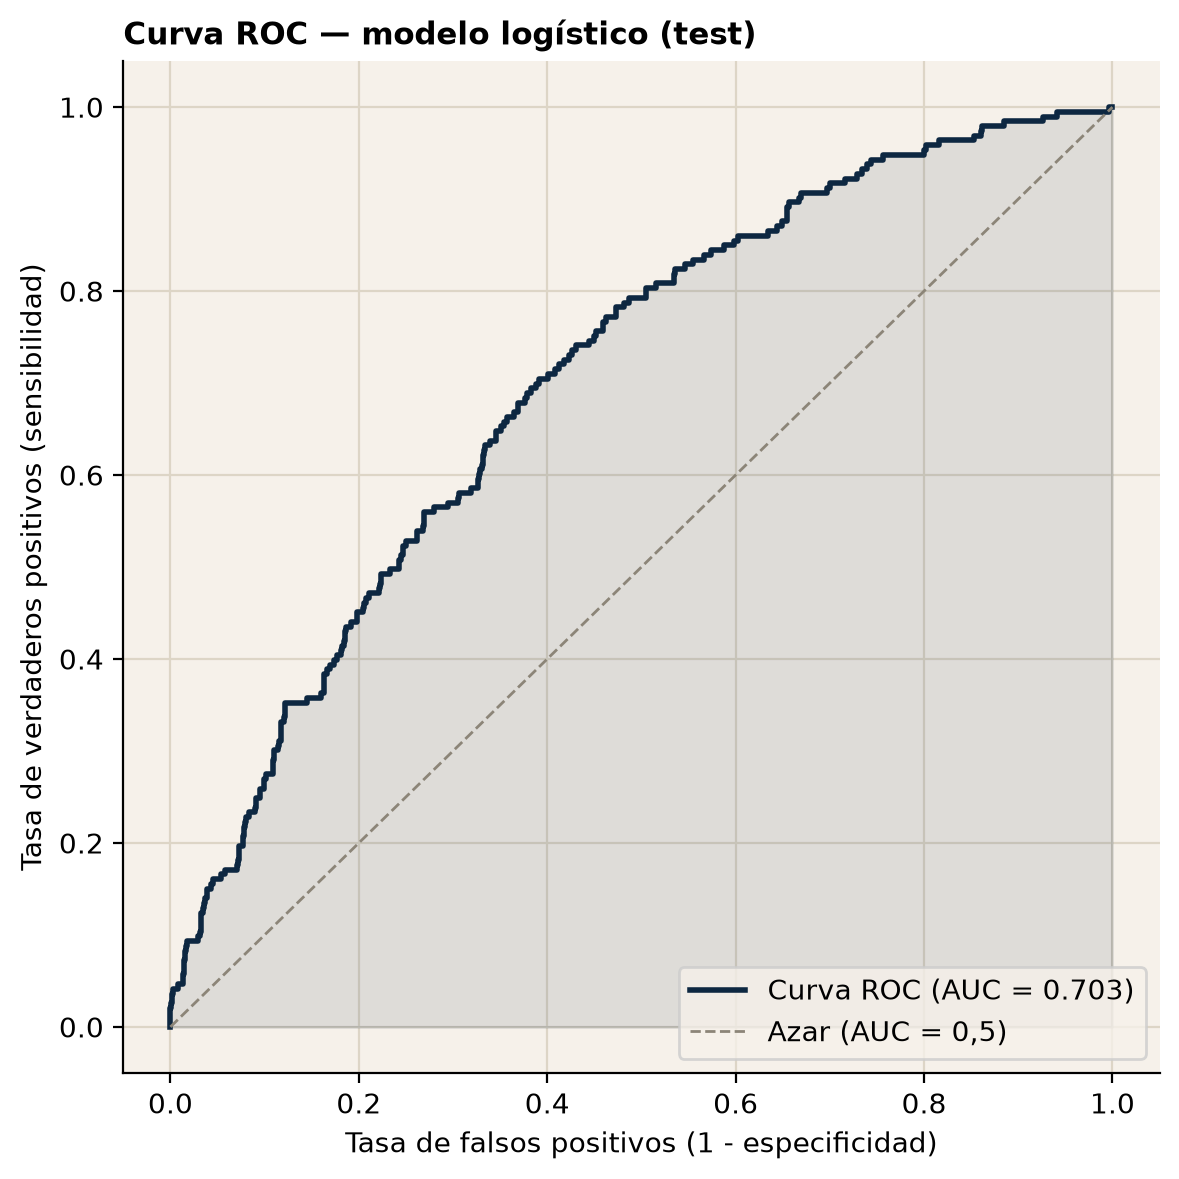
\includegraphics[width=0.55\linewidth]{figuras/fig_roc.png}
\end{center}

El AUC en test es 0,703, dentro del rango ``aceptable'' (0,7-0,8) de la escala de referencia: el modelo discrimina mejor que el azar (AUC = 0,5) pero está lejos de un desempeño ``bueno'' (0,8-0,9) o ``excelente'' ($>0,9$). Es consistente con que las correlaciones individuales de S1 fueron modestas (máximo 0,225): cinco predictores con asociaciones moderadas producen una capacidad discriminativa moderada, no alta. El AUC evalúa el modelo en todos los umbrales posibles, a diferencia de las métricas de 3.1, que dependen del umbral fijo de 0,5; ambas secciones se complementan.

\section{Síntesis y reflexión}
\guia{(15 pts) En formato Markdown (máx.\ 1 página): expliquen cómo integraron los resultados de S1 y S2, evalúen el desempeño del modelo y reflexionen sobre posibles mejoras metodológicas de cara a la Sumativa 3.}
\resp

\end{document}
